\section{Experiments}

\subsection{Protocol and Metrics}

The experiments follow a six-link evidence chain: existence, formation attribution, matched mitigation, cross-communication replication, HFL field-position comparison, and external-validity boundaries. DSA is the primary shortcut endpoint. We report it alongside operator-grid accuracy and frozen task metrics: client-average accuracy (Avg), minimum client accuracy (Worst), worst valid class--operator-cell accuracy (WCCA), and the mean within-class accuracy range across operators (CFG; lower is better). No accuracy metric is treated as a substitute for DSA.

The experiments use matched contrasts rather than a single cross-protocol leaderboard. The held-out map2 study is the main comparison of local risk objectives; map1 changes the class--operator binding while keeping the remaining controlled factors fixed; FedDF-fidelity changes the HFL communication base. Table~\ref{tab:protocol-boundary} summarizes the information available during training and evaluation.

\begin{table*}[t]
\centering
\small
\caption{Information boundary for completed and frozen comparison protocols. Operator identities and binding maps are sealed from deployable training.}
\label{tab:protocol-boundary}
\resizebox{\textwidth}{!}{%
\begin{tabular}{lllll}
\toprule
Protocol role & Private task & Train-time environment information & Communication context & Evaluation-only information \\
\midrule
CLE formation / local-first & CIFAR--10 & none & Local or strict AsymHFL & operator, binding, paired grid \\
Axis I mechanism objectives ($\alpha=.5,\rho=1,\gamma=.9$) & CIFAR--10 & none or PEW family proxy, by arm & strict AsymHFL & operator, binding, paired grid \\
Cross-binding map1 & CIFAR--10 & PEW family proxy for PEW+BER & strict AsymHFL & operator, binding, paired grid \\
Second communication base & CIFAR--10 & PEW family proxy for PEW+BER & FedDF-fidelity & operator, binding, paired grid \\
Main-evaluation dose response ($\alpha=1,\rho=.5$) & CIFAR--10 & none or PEW family proxy, by arm & strict AsymHFL & operator, binding, paired grid \\
Axis II main-evaluation context ($\alpha=1,\rho=.5,\gamma=.9$) & CIFAR--10 & method-specific; BER only in its named row & protocol-matched HFL family & operator, binding, paired grid \\
\bottomrule
\end{tabular}%
}
\end{table*}

\begin{table*}[t]
\centering
\small
\caption{Research questions, matched protocols, and evidential roles.}
\label{tab:research-questions}
\begin{tabularx}{\textwidth}{lXll}
\toprule
RQ & Question & Primary endpoint & Evidence status \\
\midrule
RQ1 & Does high-exposure CLE induce prediction shifts along the registered binding? & Paired DSA and shuffled null & complete \\
RQ2 & Does the shortcut form locally or arise mainly through communication? & HFL/Local matched DSA contrast & 3 seeds complete; 3/3 mechanism gates pass \\
RQ3 & Does class-conditional support balancing outperform matched generic reweighting? & DSA with utility reported separately & fixed-budget complete \\
RQ4 & Does suppression transfer across bindings and communication mechanisms? & Within-setting DSA delta & controlled maps/base complete \\
RQ5 & Does shortcut strength vary with \(\gamma\) under the main evaluation protocol? & DSA dose response & seed 0 complete \\
RQ6 & Do representative HFL mechanisms remove CLE on their own? & DSA plus clean/corrupt accuracy & 5/8 rows complete \\
RQ7 & What correspondence, taxonomy, and external-validity boundaries remain? & Oracle and bounded stress audits & partial \\
\bottomrule
\end{tabularx}
\end{table*}


The mechanism protocol isolates binding-directed behavior under deliberately high CLE exposure; the main evaluation protocol measures dose response and task utility under a fixed clean--corrupted mixture. Results from the two regimes are not pooled into one leaderboard.

\subsection{Local-versus-Communication Formation}

We compare four matched arms under CLE-v2: HFL with \(\gamma_{\mathrm{CLE}}=0\), HFL with \(\gamma_{\mathrm{CLE}}=0.9\), Local with \(\gamma_{\mathrm{CLE}}=0\), and Local with \(\gamma_{\mathrm{CLE}}=0.9\). All arms share the same AugMix/JSD/DCL local baseline, run for 12 rounds, and use at most 16 local batches per client per round. We repeat the complete factorial for training seeds 0/1/2 while holding the partition, binding, initialization, fit/audit/test roles, public batches, and paired evaluation grid fixed. The mechanism factorial uses its frozen 12-round budget, distinct from the 40-round held-out objective comparison.

\begin{table*}[t]
\centering
\small
\caption{DSA-based CLE formation and local-versus-communication attribution across training seeds. $\Delta_{\mathrm{comm}}=\Delta_{\mathrm{HFL}}-\Delta_{\mathrm{Local}}$. The ratio is descriptive rather than a causal mediation proportion.}
\label{tab:local-first}
\resizebox{\textwidth}{!}{%
\begin{tabular}{lrrrrl}
\toprule
Seed & $\Delta_{\mathrm{HFL}}$ & $\Delta_{\mathrm{Local}}$ & $\Delta_{\mathrm{comm}}$ & Local/HFL (\%) & DSA mechanism gates \\
\midrule
0 & 0.119889 & 0.107960 & 0.011929 & 90.05 & 3/3 pass \\
1 & 0.123717 & 0.127287 & -0.003570 & 102.89 & 3/3 pass \\
2 & 0.124638 & 0.131210 & -0.006573 & 105.27 & 3/3 pass \\
\midrule
Mean $\pm$ SD & $0.122748\pm0.002518$ & $0.122152\pm0.012446$ & $0.000596\pm0.009929$ & $99.40\pm8.19$ & 3/3 seeds \\
\bottomrule
\end{tabular}%
}
\end{table*}


Figure~\ref{fig:local-first} visualizes both matched contrasts and the communication difference for each training seed.

\begin{figure*}[t]
\centering
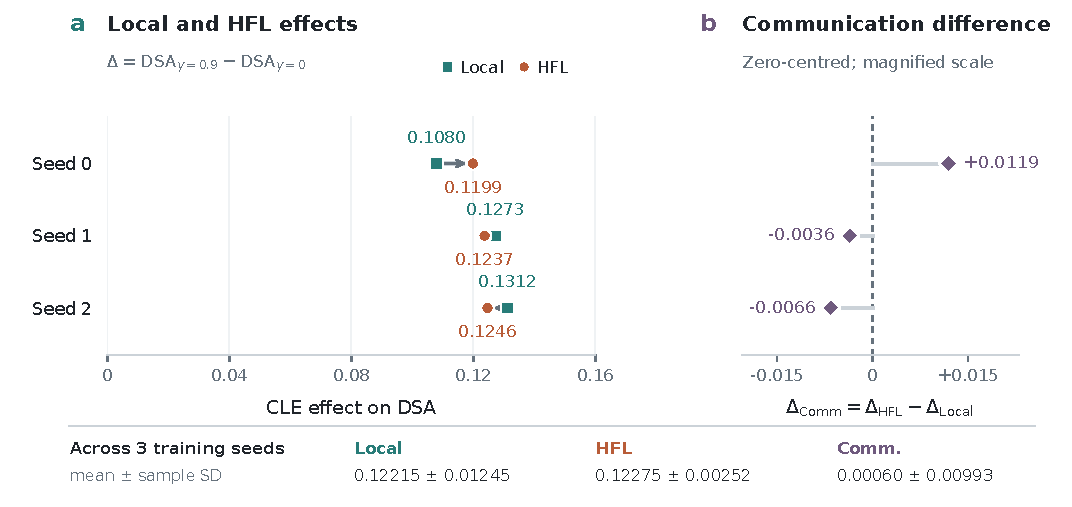
\includegraphics[width=0.96\textwidth,keepaspectratio]{figures/fig_local_first_multiseed_v1.pdf}
\caption{Local-first formation across three matched training seeds. (a) The CLE effect is the DSA contrast between $\gamma=0.9$ and $\gamma=0$ under HFL or Local training; paired endpoints share the same training seed. (b) Their communication difference is shown on a magnified zero-centred axis. Bottom summaries report the mean and sample SD across training seeds. The mechanism factorial uses its frozen 12-round, 16-local-batch budget.}
\label{fig:local-first}
\end{figure*}

Across seeds 0/1/2, \(\Delta_{\mathrm{HFL}}\) is
\(0.122748\pm0.002518\) and \(\Delta_{\mathrm{Local}}\) is
\(0.122152\pm0.012446\) (mean \(\pm\) sample standard deviation). The corresponding
\(\Delta_{\mathrm{comm}}=\Delta_{\mathrm{HFL}}-\Delta_{\mathrm{Local}}\) values are
\(0.011929\), \(-0.003570\), and \(-0.006573\), giving
\(0.000596\pm0.009929\). Thus the large Local contrast reproduces in every seed,
whereas the communication difference is small on average and not sign-stable. All three seeds pass the directional-shortcut, binding-specificity, and local-first DSA gates. We call this pattern \textbf{predominantly local-first formation}. Ratios such as \(\Delta_{\mathrm{Local}}/\Delta_{\mathrm{HFL}}\) remain descriptive rather than per-example mediation quantities or claims that communication is irrelevant.

\subsection{Axis I: Matched Shortcut-Objective Attribution}

A five-arm 12-round screen was used for method selection only. JTT therefore remains screening-only and is not part of the Formal comparison. Axis I uses the mechanism protocol on held-out map2 ($\alpha=0.5$, $\rho=1.0$, and $\gamma=0.9$) and compares four matched arms: ERM, protocol-matched CVaR-DRO, PEW+GroupDRO, and PEW+BER. The arms share the partition, training and evaluation seeds, initial states, private batch trajectory, and strict HFL communication protocol. PEW+GroupDRO and PEW+BER also receive identical PEW group assignments. This design asks whether BER's class-conditional support balancing matters beyond generic tail emphasis or worst-group optimization. DSA is the primary endpoint; utility is reported separately and is not interpreted as ordinary clean-CIFAR performance under this deliberately high-exposure mechanism test.

\begin{table*}[t]
\centering
\small
\caption{Completed held-out-map2 objective comparison over training seeds 0/1/2 (mean $\pm$ sample standard deviation). All arms use the same disclosed fixed local-batch budget and establish mechanism-level separation.}
\label{tab:map2-methods}
\resizebox{\textwidth}{!}{%
\begin{tabular}{lrrrrrr}
\toprule
Arm & DSA $\downarrow$ & Operator-grid Acc. $\uparrow$ & Last-10 Avg $\uparrow$ & Last-10 Worst $\uparrow$ & WCCA $\uparrow$ & CFG $\downarrow$ \\
\midrule
ERM & $0.2505\pm0.0087$ & $20.4950\pm0.3718$ & $19.9589\pm0.1212$ & $16.3780\pm0.1259$ & $0.0000\pm0.0000$ & $32.7467\pm0.1708$ \\
CVaR-DRO & $0.0867\pm0.0055$ & $19.2206\pm1.1055$ & $18.5788\pm0.3102$ & $14.2636\pm0.2640$ & $0.1167\pm0.0629$ & $27.6750\pm0.1885$ \\
\ifdraftskeleton
JTT Formal & \pendingcell & \pendingcell & \pendingcell & \pendingcell & \pendingcell & \pendingcell \\
\fi
PEW+GroupDRO & $0.2054\pm0.0080$ & $21.4517\pm0.5783$ & $20.9963\pm0.0924$ & $17.5309\pm0.5148$ & $0.0333\pm0.0144$ & $31.8950\pm0.9747$ \\
\textbf{PEW+BER} & $\mathbf{0.0715\pm0.0113}$ & $\mathbf{25.1772\pm1.2522}$ & $\mathbf{24.5466\pm0.1098}$ & $\mathbf{20.7516\pm0.6126}$ & $\mathbf{2.6500\pm0.0750}$ & $\mathbf{22.7825\pm0.5428}$ \\
\bottomrule
\end{tabular}%
}
\ifdraftskeleton
\par\smallskip
JTT remains screening-only; its row should be populated only if a formal JTT comparison is later authorized and completed.
\fi
\end{table*}


Figure~\ref{fig:axis1-objectives} jointly displays the primary shortcut endpoint and operator-grid accuracy. It makes the central distinction explicit: a method can reduce DSA without occupying the same position on the utility axis.

\begin{figure*}[t]
\centering
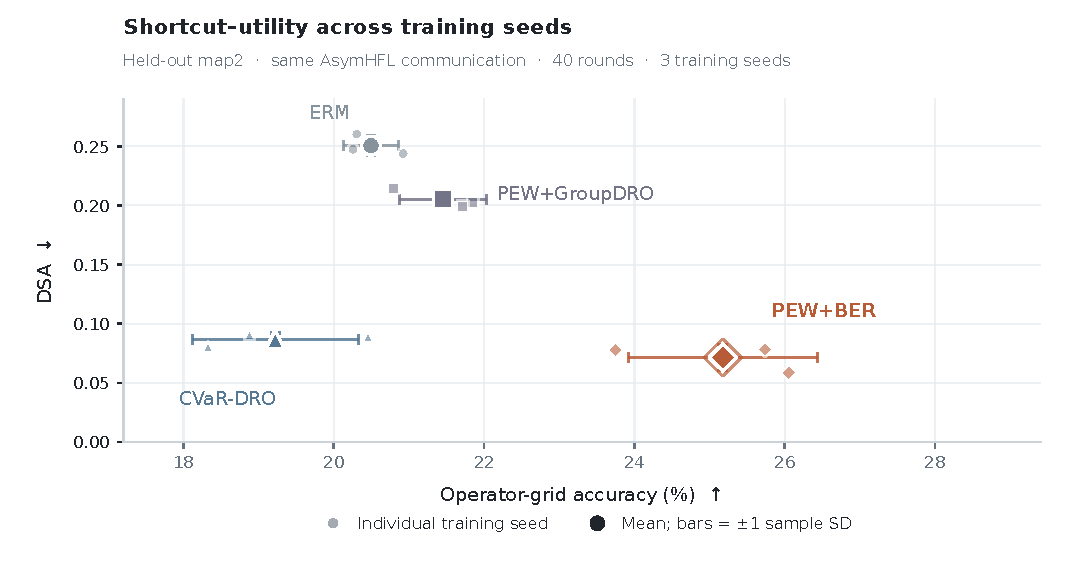
\includegraphics[width=0.94\textwidth,keepaspectratio]{figures/fig_objective_tradeoff_v2.pdf}
\caption{Shortcut--utility comparison on held-out map2 under the mechanism protocol. Small markers denote individual training seeds and large markers their means. Horizontal and vertical bars show one sample SD for operator-grid accuracy and DSA, respectively. All four local objectives use matched 40-round, 16-local-batch budgets and the same AsymHFL communication.}
\label{fig:axis1-objectives}
\end{figure*}

The completed fixed-budget study gives the following source-paired differences for training seed 0:

\[
\mathrm{DSA(ERM)}-\mathrm{DSA(BER)}=0.182567,
\]

with 95\% interval \([0.180596,0.184407]\),

\[
\mathrm{DSA(GroupDRO)}-\mathrm{DSA(BER)}=0.136834,
\]

with \([0.134952,0.138706]\), and

\[
\mathrm{DSA(BER)}-\mathrm{DSA(CVaR)}=-0.011240,
\]

with \([-0.012355,-0.010092]\). These intervals resample semantic sources conditional on the seed-0 checkpoints.

Across training seeds 0/1/2 in that protocol, DSA(ERM)$-$DSA(BER) is \(0.179060\pm0.008594\), and DSA(GroupDRO)$-$DSA(BER) is \(0.133947\pm0.011518\); both contrasts favor BER in all three seeds. DSA(BER)$-$DSA(CVaR) is \(-0.015184\pm0.015411\), while BER improves operator-grid accuracy over CVaR by \(5.9567\pm2.3151\) percentage points. The pre-registered fixed-budget multi-seed gates pass. These results establish the controlled mechanism comparison under its disclosed local-batch budget; we do not mix it with the separate main evaluation protocol.

The shared-PEW comparison separates access to PEW groups from the BER objective: PEW+GroupDRO retains pooled DSA \(0.2054\pm0.0080\), whereas PEW+BER reaches \(0.0715\pm0.0113\). CVaR-DRO is closer at \(0.0867\pm0.0055\). BER has higher pooled operator-grid accuracy, Avg, Worst, and WCCA, and lower CFG in the same fixed-budget study. The per-client ordering is mixed: CVaR-DRO is lower on c0 and c1, while BER is lower on c2 and c3. The supported conclusion is therefore pooled and protocol-specific, not per-client dominance.

\subsection{Cross-Binding and Cross-Communication Validation}

Table~\ref{tab:cross-setting-dataset} summarizes completed PEW+BER comparisons on the original binding map, map1, and FedDF-fidelity. A second private dataset remains a separate evidence slot.

\begin{table*}[t]
\centering
\small
\caption{Within-setting PEW+BER comparisons across binding maps and communication bases.}
\label{tab:cross-setting-dataset}
\resizebox{\textwidth}{!}{%
\begin{tabular}{lllrrrr}
\toprule
Private task & Binding / protocol & HFL base & Base DSA & PEW+BER DSA & Relative reduction & Avg delta \\
\midrule
CIFAR--10 & original map & Asymmetric HFL & 0.119644 & 0.041252 & 65.52\% & +1.7323 \\
CIFAR--10 & map1 & Asymmetric HFL & 0.113761 & 0.049531 & 56.46\% & +0.7040 \\
CIFAR--10 & held-out map2, fixed budget (3 seeds) & Asymmetric HFL & 0.250530 & 0.071470 & 71.47\% & +4.5877 \\
CIFAR--10 & original map & FedDF-fidelity & 0.136989 & 0.029012 & 78.82\% & -0.6660 \\
\ifdraftskeleton
Second private task & dataset/protocol pending & pending & \pendingcell & \pendingcell & \pendingcell & \pendingcell \\
\fi
\bottomrule
\end{tabular}%
}
\ifdraftskeleton
\par\smallskip
The FedDF-fidelity row supports cross-communication shortcut suppression but not a universal utility gain. \evidenceneeded{second private dataset; dataset and protocol pending.}
\fi
\end{table*}


On map1, only the client-specific class--operator binding changes; the partition, evaluation seed, training seed, initial weights, public data, evaluation grid, and frozen PEW remain fixed. Pooled DSA changes from \(0.113761\) to \(0.049531\), a 56.46\% reduction, and all four clients move in the same direction. Operator-grid accuracy changes from \(20.9450\%\) to \(21.4583\%\). This reproduces DSA suppression on a second controlled binding direction at seed 0.

The completed second communication-base experiment uses native single-view CE with a protocol-matched \textbf{FedDF-fidelity} adapter. Base and BER arms share initialization, private batches, public distillation, and training budget. Pooled DSA changes from \(0.136989\) to \(0.029012\), while operator-grid accuracy changes by \(-0.0400\) points and last-five Avg by \(-0.6660\) points. The frozen utility gate fails, and both arms fall below the pre-registered 20\% operator-grid learning floor. We use this experiment as boundary evidence that DSA suppression can appear under another communication mechanism; it does not establish cross-base utility gain.

To test the stronger mechanism-level question under a classic and computationally light communication rule, a pending FedMD replication holds communication fixed across the same four local objectives used in the main comparison. This experiment is a controlled cross-communication replication, not a claim that PEW+BER is universally compatible with every HFL algorithm.

\evidenceneeded{second private dataset; dataset and protocol pending.}

\subsection{Dose Response and Utility under the Main Evaluation Protocol}

The mechanism protocol intentionally combines stronger label skew, corruption of every private image, and strong class--operator binding to maximize shortcut identifiability. The complementary main evaluation protocol keeps the private task and held-out binding map fixed while using Dirichlet $\alpha=1.0$, private corruption rate $\rho=0.5$, and $\gamma\in\{0,0.5,0.9\}$. This clean--corrupted mixture permits DSA and task utility to be assessed together; it is not introduced as a replacement for the mechanism protocol. For sample $i$ at client $k$, a fixed corruption indicator $C_{ki}\sim\mathrm{Bernoulli}(\rho)$ is shared across all three $\gamma$ conditions. Conditional on $C_{ki}=1$,
\[
P(E=e\mid Y=c,k,C=1)=\frac{1-\gamma}{11}+\gamma\mathbf{1}[e=b_k(c)].
\]
Sources, labels, corruption masks, severities, fit/audit splits, model initialization, public data, and the paired operator grid are held fixed. Thus $\alpha$ controls client label support, $\rho$ controls exposure to corruption, and $\gamma$ controls class-conditional operator concentration. This is a complementary controlled evaluation on CIFAR--10, not a second private dataset.

\ifdraftskeleton
\begin{table}[t]
\centering
\small
\caption{Dose response under the main evaluation protocol at training seed 0. The corruption mask, partition, sources, severities, initialization, and evaluation grid are paired across $\gamma$.}
\label{tab:moderate-dose}
\resizebox{\columnwidth}{!}{%
\begin{tabular}{llrrrr}
\toprule
$\gamma$ & Objective & DSA $\downarrow$ & Operator Acc. $\uparrow$ & Clean Acc. $\uparrow$ & Mixed Acc. $\uparrow$ \\
\midrule
0.0 & ERM & -0.0007 & 48.480 & 52.325 & 50.089 \\
0.5 & ERM & 0.0397 & 48.395 & 54.350 & 51.140 \\
0.9 & ERM & 0.1845 & 37.193 & 49.700 & 43.354 \\
0.9 & PEW+BER & 0.0900 & 38.160 & 45.350 & 41.562 \\
\bottomrule
\end{tabular}%
}
\end{table}
\fi


Figure~\ref{fig:dose-response} shows the measured dose response and the task-utility changes of the matched intervention.

\begin{figure*}[t]
\centering
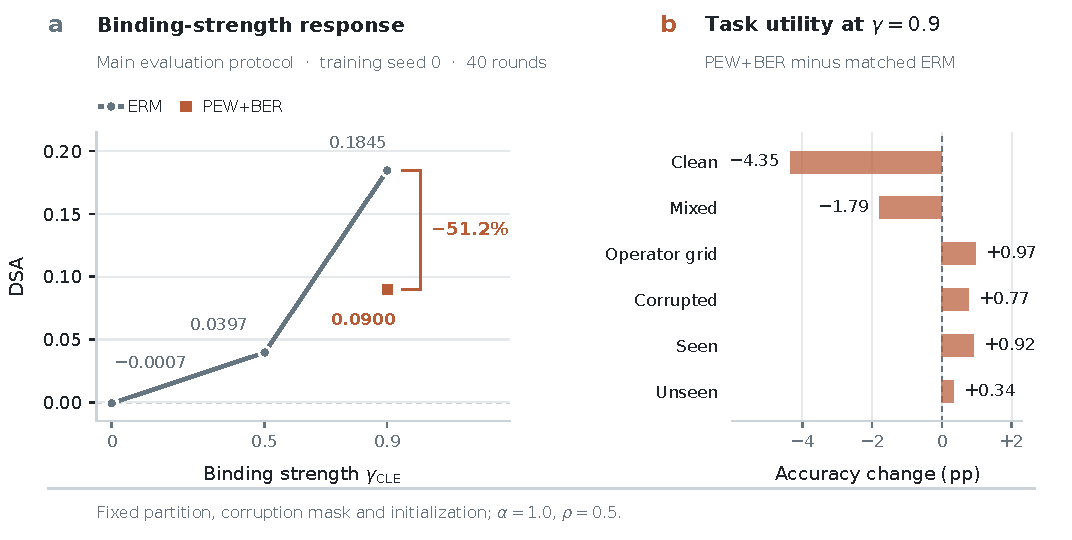
\includegraphics[width=0.96\textwidth,keepaspectratio]{figures/fig_dose_response_v3.pdf}
\caption{Binding-strength response and task utility under the main evaluation protocol at training seed 0. (a) Lines connect the three measured ERM settings. The matched PEW+BER intervention is evaluated only at $\gamma=0.9$, where DSA is reduced by 51.2\%. (b) Candidate-minus-control accuracy changes include improvements on corrupted evaluations and declines on clean and mixed evaluations. This experiment uses 40 rounds with 64 local batches per client per round.}
\label{fig:dose-response}
\end{figure*}

Under ERM, DSA increases from \(-0.000730\) at \(\gamma=0\) to \(0.039679\) at \(\gamma=0.5\) and \(0.184514\) at \(\gamma=0.9\). Source-paired bootstrap intervals for both adjacent increments exclude zero, while the \(\gamma=0\) estimate does not exceed its shuffled-binding null. The response is therefore monotone in this controlled seed, although we do not assume linearity in \(\gamma\). At \(\gamma=0.9\), PEW+BER lowers DSA to \(0.090024\), but the residual remains above its shuffled-binding null.

\subsection{Axis II: HFL Mechanism-Family Context}

Axis II asks a different question from the matched objective study: whether representative heterogeneous-FL communication and robustness mechanisms naturally remove CLE while retaining usable task semantics. The pre-specified eight-row main table contains Local/ERM, FedMD, FedProto, FedDF, AugHFL, RAHFL, AsymHFL--ERM, and AsymHFL+PEW+BER. All final rows use the main evaluation protocol on held-out map2 ($\alpha=1.0$, $\rho=0.5$, $\gamma=0.9$), training seed 0, the same 40-round budget, initial states, and paired operator evaluation grid. Ordinary HFL mechanisms and corruption-robust AugHFL/RAHFL are retained because communication robustness, corruption robustness, and directional-shortcut suppression are distinct capabilities. We report DSA together with paired-grid, clean-subset, corrupted-subset, and overall task accuracy; per-client DSA and Worst/WCCA/CFG remain in the detailed analysis. Existing mechanism-protocol Local/FedMD runs are internal engineering records and do not enter the paper tables.

\ifdraftskeleton
\begin{table*}[t]
\centering
\small
\caption{Protocol-matched HFL mechanism-family context under the main evaluation protocol on held-out map2 ($\alpha=1.0$, $\rho=0.5$, and $\gamma=0.9$; Axis II). Five rows are completed seed-0 Formal results; remaining cells are pending.}
\label{tab:hfl-context}
\resizebox{\textwidth}{!}{%
\begin{tabular}{llllrrrrr}
\toprule
Method & Model heterogeneity & Local robustness & Communication & DSA $\downarrow$ & Grid Acc. $\uparrow$ & Clean Acc. $\uparrow$ & Corrupt Acc. $\uparrow$ & Mixed Acc. $\uparrow$ \\
\midrule
Local/ERM & yes & none & none & 0.168374 & 39.830 & 51.425 & 39.508 & 45.467 \\
FedMD adapter & yes & none & public-logit exchange & 0.167835 & 38.732 & 50.400 & 38.378 & 44.389 \\
FedProto adapter & yes & none & class prototypes & 0.160788 & 39.250 & 50.800 & 38.937 & 44.868 \\
FedDF-fidelity & yes & none & public distillation & \pendingcell & \pendingcell & \pendingcell & \pendingcell & \pendingcell \\
AugHFL-fidelity & yes & AugMix/JSD & heterogeneous collaboration & \pendingcell & \pendingcell & \pendingcell & \pendingcell & \pendingcell \\
RAHFL anchor & yes & AugMix/JSD/DCL & asymmetric collaboration & \pendingcell & \pendingcell & \pendingcell & \pendingcell & \pendingcell \\
AsymHFL--ERM & yes & none & strict asymmetric collaboration & 0.184514 & 37.193 & 49.700 & 37.008 & 43.354 \\
AsymHFL+PEW+BER & yes & class-conditional environment balancing & strict asymmetric collaboration & 0.090024 & 38.160 & 45.350 & 37.773 & 41.562 \\
\bottomrule
\end{tabular}%
}
\par\smallskip
The eight-row main table was fixed before results were observed. Existing mechanism-protocol Local/FedMD and all smoke/benchmark outputs are engineering records only and are excluded. In the matched AsymHFL pair, PEW+BER reduces DSA but does not preserve clean or mixed utility; no complete ranking claim is made while three rows remain pending.
\end{table*}
\fi


Five Formal rows are complete. Local/ERM, FedMD, and FedProto have pooled DSA values of \(0.168374\), \(0.167835\), and \(0.160788\), respectively; all exceed the shuffled-binding null. FedMD is statistically indistinguishable from Local in the paired DSA contrast, while FedProto produces a small DSA reduction of \(0.007587\) (4.51\%) with slightly lower utility. In the exactly batch-matched AsymHFL pair, PEW+BER reduces DSA from \(0.184514\) to \(0.090024\) (51.21\%), with a source-paired 95\% interval of \([0.091877,0.097081]\) for the control-minus-method contrast and reductions on all four clients. Grid and corrupted accuracy improve by \(0.967\) and \(0.765\) points, respectively, whereas clean and 50/50 mixed accuracy fall by \(4.350\) and \(1.793\) points. These rows show substantial shortcut suppression with a nonuniform utility trade-off; they are not a complete ranking of the eight methods.

\evidenceneeded{remaining main-evaluation held-out-map2 Formal rows: FedDF-fidelity, AugHFL, and RAHFL.}

\subsection{Environment Correspondence and Granularity}

A non-deployable Oracle audit compares true family grouping, true operator grouping, and a random operator correspondence. Random operator DSA exceeds Oracle operator DSA by \(0.052112\), with source-bootstrap 95\% interval \([0.051231,0.052983]\), showing that the environment correspondence matters in this audit. The Oracle family--operator DSA gap is \(0.001449\), with \([0.001086,0.001790]\). The small granularity gap is specific to this controlled audit and provides no empirical reason to introduce an operator-level PEW in the current paper. Appendix C reports the complete Oracle table.

\subsection{Remaining Evidence Placeholders}

The internal manuscript keeps unresolved evidence visible. The existing three-seed mechanism-protocol objective comparison is a completed fixed-budget study; its numbers must not be mixed with the abandoned higher-budget rerun. The local-first factorial is now complete for training seeds 0/1/2, and all three pass the directional-shortcut, binding-specificity, and local-first DSA gates. Five main-evaluation HFL-context rows and the seed-0 dose response are complete, while FedDF-fidelity, AugHFL, and RAHFL remain open. Additional gaps are a genuinely second private dataset, a bounded taxonomy stress test, and the FedMD four-objective replication. A JTT Formal is optional and is required only if the final paper makes a direct empirical superiority claim over JTT.

\evidenceneeded{bounded taxonomy stress test; protocol pending.}
